\documentclass{article}[12pt]
\usepackage[utf8x]{inputenc}

\usepackage{url} \urlstyle{sf}
\usepackage[a4paper,margin=1.9cm]{geometry}
\usepackage{xspace}
%\usepackage[american]{babel}
\usepackage{palatino}
\usepackage{bibtopic}
%\usepackage{boxit}
\usepackage{RR}
\usepackage{hyperref}
\usepackage{color}

%\usepackage{enumitem}
%\usepackage{dot2texi}


\newcommand{\refpage}[1]{\ref{#1} page~\pageref{#1}}

\newcommand{\kaapi}{\textsc{X}-Kaapi\xspace}
%%%\newcommand{\new}{\hspace*{10ex}\textbf{\textsc{New in \kaapi.}~\\}\xspace}
%\newcommand{\new}{}
%\newcommand{\inote}[1]{\textit{\textbf{  \center \hrule Implementation note\hrule}}\vspace*{1ex}\textit{#1}\vspace{1ex} \hrule
%\vspace*{2ex}}

%%\newcounter{subsubsection}[subsection]
%\renewcommand{\subsubsection}[1]{~\\ \addtocounter{subsubsection}{1} \noindent\textit{
%%\textbf{\thesubsection.
%\thesubsubsection. #1\\}}

%
%\newcounter{subsubsubsection}[subsubsection]
%\newcommand{\subsubsubsection}[1]{~\\ \addtocounter{subsubsubsection}{1} \noindent\textit{\textbf{\thesubsubsection.
%\thesubsubsubsection. #1\\}}}
%\newtheorem{proposition}{Proposition}

%%\renewcommand{\subsubsection}[1]{~\\ \addtocounter{subsubsection}{1} \noindent\textit{\textbf{\thesubsubsection\hspec #1\\}}}

\begin{document}

\RRdate{November 2011}
\RRauthor{
Thierry Gautier
\and
Jo\~{a}o V. F. Lima
}
\RRtitle{\kaapi Tracing Tool}
\RRabstract{}
\RRresume{}
\RRmotcle{}
\RRkeyword{}
\RRprojets{MOAIS}
\RCGrenoble
\RRNo{}

\makeRT % cas d'un rapport technique.

\newpage
\tableofcontents
\newpage

\section*{Foreword}

\kaapi is developed by the INRIA MOAIS team \url{http://moais.imag.fr}.
The \kaapi project is still under development.  We do our best to produce as
good documentation and  software as possible.  
Please inform us of any bug, malfunction, question, or comment. \\ 
~\\
~\\
This documentation presents the \kaapi trace utilities. \kaapi is a library with several APIs. 
The C interface is the lowest interface to program directly on top of the
runtime. The C++ interface is an extension of Athapascan-1 interface with new
features to avoid explicit declaration of shared variable.
\kaapi may also be used with C++ through a parallel STL implementation.

\section*{About \kaapi}

\kaapi  is a \textbf{``high level''}  interface in the sense that no reference is made to the execution support.  
The synchronisation, communication, and scheduling of operations are fully controlled by the software. 
   \kaapi is an  \textbf{explicit parallelism language}: the programmer indicates the parallelism of the algorithm through \kaapi's one, easy-to-learn  template functions, \texttt{Spawn} to create tasks.   The programming semantics are similar to those of a sequential 
 execution in that each ``read'' executed in parallel returns the value it would have returned had the ``read'' been executed  sequentially. 
 
The following documentations exist about \kaapi:
\begin{itemize}
\item \kaapi comes from Athapascan interface defined in 1998 and updated in the INRIA technical report RT-276. Available at: \url{http://hal.inria.fr/inria-00069901}.
\item The INRIA RT-417 presents the C API. Available at: \url{http://hal.inria.fr/hal-00647474}.
\item The INRIA RT-418 presents the KaCC compiler that allows to write parallel program using code annotation with pragma. Available at: \url{http://hal.inria.fr/hal-00648245}.
\end{itemize}
\kaapi is composed by one runtime and several application programming interfaces (API).
All these APIs are based on the runtime functions. With specific options it is
possible to create a version of the library that is able to record events at
runtime, and then to process them to display Gantt diagram or to have access to
some statistics.


% ---------------------------------------------------------------
\section*{Reading this Document}
% ---------------------------------------------------------------
This document is a developer documentation designed to describe how to use the
\kaapi's trace utilities. If the reader can not find its information into this
document, please refer to the \kaapi web site at
\url{http://kaapi.gforge.inria.fr}.

This document is organised as following:
\begin{itemize}
\item The configuration options required to configure and install \kaapi,
as well as to generate execution traces, is describe in Section~\ref{sec:userinstall};
\item Section~\ref{sec:generate} describes how to generate \kaapi traces;
\item Section~\ref{sec:convert} presents how to convert internal binary
representation of events to the Paj\'e trace format;
\item Section~\ref{sec:visualisation} describes visualisation details of \kaapi traces, which
can be displayed using ViTE or Paj\'e;
\item The display of PAPI performance counters is given in Section~\ref{sec:papi}.
\end{itemize}


% ---------------------------------------------------------------
\newpage
\section{Software installation}\label{sec:userinstall}
% ---------------------------------------------------------------

\kaapi is both a programming model and a runtime for high performance parallelism targeting multicore and distributed architectures. 
It relies on the work stealing paradigm.
\kaapi was developed in the MOAIS INRIA project by Thierry Gautier, Fabien Le Mentec, Vincent Danjean, and Christophe Laferrière in the early stage of the library.

\subsubsection*{\kaapi Contacts}
If you wish to contact the XKaapi team, please visit the web site at:
\begin{center}
\url{http://kaapi.gforge.inria.fr}
\end{center}

\subsection{Supported Platforms}

\kaapi targets essentially SMP and NUMA platforms. The runtime should run
on any system providing:
\begin{itemize}
\item a GNU toolchain ($\textrm{GCC} \ge 4.3$);
\item the pthread library;
\item Unix-based environment.
\end{itemize}
It has been extensively tested on the following operating systems:
\begin{itemize}
\item GNU-Linux with x86\_64 architectures;
\item Mac OS X with Intel processors.
\end{itemize}
NVIDIA GPU support has been tested on the following configurations:
\begin{itemize}
\item NVIDIA's Fermi and Kepler GPUs;
\item CUDA Toolkit 5.0 and 4.2.
\end{itemize}
There is no version for Windows yet.

\subsection{\kaapi library installation}

To install \kaapi programming environment, you need to:
\begin{itemize}
\item compile the \kaapi library;
\item install the \kaapi library.
\end{itemize}
The \kaapi libraries and runtime are available at \url{http://kaapi.gforge.inria.fr} (tarball). \kaapi libraries and runtime are distributed under a CeCILL-C license\footnote{\url{http://www.cecill.info/index.en.html} for english version}:
\begin{center}
\begin{minipage}{0.9\linewidth}
\it
CeCILL-C is well suited to libraries and more generally software components. Anyone distributing an application which includes components under the CeCILL-C license must mention this fact and make any changes to the source code of those components available to the community under CECILL-C while being free to choose the licence of its application.\end{minipage}
\end{center}

Currently, \kaapi must be installed from sources. 
Other packagings (Debian or RPM packages) are under development. Please visit the \kaapi web site for an up-to-date information:
\begin{center}
\url{http://kaapi.gforge.inria.fr}
\end{center}

%There are 2 ways to install \kaapi:
%\begin{itemize}
%\item using the Debian packages,
%\item installing from source.
%\end{itemize}
%
%%% sub
%\subsubsection*{Using the Debian packages}
%Below is a list of the Debian packages provided for using and programming with \kaapi. \\
%\textit{
%TODO: décrire ici le package nécessaire pour le compilateur. A priori uniquement la lib C + éventuellement une lib C++ pour des classes tableaux et/ou autre data structure qui serait déjà 'pré-définie' pour être passer correctement en paramètre de tâche. Je pense ici à la lib des array/range2D qui permet facilement de faire de la découpe récursive de données.
%}
%%% sub
\subsubsection*{Installing from sources}

There are 2 ways to retrieve the sources:
\begin{itemize}
\item download a release snapshot at the following url:\newline
\url{https://gforge.inria.fr/frs/?group_id=94}.
\item clone the master branch of the git repository of the project:\newline
\verb+> git clone git://scm.gforge.inria.fr/kaapi/xkaapi.git xkaapi+
\end{itemize}


\paragraph{Configuration.}
The build system uses GNU Autotools.
In case you cloned the project repository, you first have to bootstrap the
configuration process by running the following script:
\begin{verbatim}
> ./bootstrap
\end{verbatim}
The \textit{configure} file is used to create the
\textit{Makefile} accordingly to your system configuration. Command line
options can be used to modify the default behaviour. A list of the
configuration options is available by running:
\begin{verbatim}
> ./configure --help
\end{verbatim}

The options related to \kaapi trace support are:
\begin{itemize} %% option list
\item \verb+--enable-mode=debug+ or \verb+release+\newline
Choose the compilation mode of the library. Defaults to release.
\item \verb+--with-cuda=<CUDA installation>+\newline
Enable CUDA GPU execution support.
\item \verb+--with-perfcounter+\newline
Enable performance counters support.
\item \verb+--with-papi+\newline
Enable the PAPI library for low level performance counting.
More information on PAPI can be found at \url{http://icl.cs.utk.edu/papi}.
\item \verb+--with-poti+\newline
(Optional) Specify an external up-to-date POTI library to generate Paj\'e traces.
More information on POTI can be found at \url{https://github.com/schnorr/poti}. 
\item \verb+--with-cupti+\newline
Enable CUPTI profiler to generate CUDA GPU traces. 
\textbf{Note}: CUDA support is required.
\item \verb+--prefix=+\newline
Overload the default installation path.
\end{itemize} %% option list
Example:

\begin{verbatim}
> ./configure --enable-mode=release --prefix=$HOME/install
> ./configure  --prefix=$HOME/install --enable-mode=release \
         --with-cuda=/usr/local/cuda-5.0 \
         --with-cupti=/usr/local/cuda-5.0/extras/CUPTI \
         --with-perfcounter 
\end{verbatim}
If there are errors during the configuration process, you have to solve
them before going further. If dependencies are missing on your
system, logs will give you the names of the software to install.

\paragraph{Compilation and installation.}
On success, the configuration process generates a Makefile. The 2 following
commands build and install the \kaapi runtime:
\begin{verbatim}
> make
> make install
\end{verbatim}

\paragraph{Checking the installation.}
The following checks that the runtime is correctly installed on your system:
\begin{verbatim}
> make check
\end{verbatim}

\paragraph{Compilation of the examples.}
The following compiles the sample applications:
\begin{verbatim}
> cd examples; make examples
\end{verbatim}

\subsubsection*{Installation directory}

The configure, make, make install, commands create in the prefix directory the following 
directory structure:
\begin{verbatim}
<prefix>/include
<prefix>/lib
<prefix>/bin
<prefix>/share
\end{verbatim}

The \texttt{<prefix>/share} directory contains some documentation and examples.

% ---------------------------------------------------------------
\section{Generating \kaapi trace files} \label{sec:generate}
% ---------------------------------------------------------------

Execution of a \kaapi program is controlled by environment variables.
For instance, \verb+KAAPI_CPUCOUNT+ and \verb+KAAPI_CPUSET+ are used
to control the number and the location of cores on the machine.

With the options presented in the previous configuration, \kaapi runtime is able to record events that corresponds to different activities at runtime. 

The record of events is enable if the environment variable \verb+KAAPI_RECORD_TRACE+ is set.
Once configured, the execution of any \kaapi program will record events such that:
\begin{itemize} 
\item one file \verb+/tmp/events.<username>.<coreid>.evt+ is created for each core of the  selected set (using \verb+KAAPI_CPUCOUNT+ or \verb+KAAPI_CPUSET+). 
\item A file \verb+/tmp/events.<username>.<coreid>.evt+ contains the sequence of events generated by the core \verb+<coreid>+ during its execution. 
\end{itemize} 

Note that for multi-GPU executions, the file names follow the same file name convention.

\subsection{Event selection}

The \kaapi runtime only records events defined into the event mask, which is
formed by a string containing three groups.
By default the event mask contains all events. The user may change it  by setting the environment variable \verb+KAAPI_RECORD_MASK+. For instance:
\begin{verbatim}
> KAAPI_RECORD_MASK="compute"
\end{verbatim}
specifies the event mask to contains only the events associated with computations.\\

The set of all events are clustered into three main classes:
\begin{itemize}
\item \textbf{compute}: which contains all  events that are associated with computations;
\item \textbf{idle}: which contains all events that are associated with idle state;
\item \textbf{steal}: that defines all events involved during work stealing operation.
\end{itemize}
These names may be used into the event mask. For instance:
\begin{verbatim}
> KAAPI_RECORD_MASK="compute,idle,steal"
\end{verbatim}
specifies an event mask that contains all events from the compute set, the idle set and steal set.

% ---------------------------------------------------------------
\section{Converting \kaapi trace files to Paj\'e format} \label{sec:convert}
% ---------------------------------------------------------------

The \kaapi \texttt{katracereader} converts internal traces in binary format
into Paj\'e trace format:
\begin{verbatim}
> katracereader <options> /tmp/events.<username>.*
\end{verbatim}
Its options are:
\begin{itemize} %% option list
\item \verb+--paje+\newline
Convert \kaapi trace files into Paj\'e format and create the output file \texttt{paje-gantt.trace}.
\item \verb+--vite+\newline
Convert \kaapi trace files into Paj\'e format compatible with ViTE and create the output file \texttt{vite-gantt.trace}.
\item \verb+--steal-event+\newline
Output steal events in the conversion process. Disabled by default.
\item \verb+--gpu-trace+\newline
Output GPU thread events of kernel executions. Disabled by default.
\item \verb+--gpu-transfer+\newline
Ouput GPU memory transfers of each GPU thread. Disabled by default.
\item \verb+--display-data+\newline
Print events to standard output.
\end{itemize} %% option list

% ---------------------------------------------------------------
\section{\kaapi Trace visualisation} \label{sec:visualisation}
% ---------------------------------------------------------------

Paj\'e trace format can be displayed using:
\begin{itemize}
\item ViTE Trace Explorer 1.2 available at \url{http://vite.gforge.inria.fr}.
\item Paj\'e visualisation tool available at \url{http://paje.sf.net}.
\end{itemize}

Figure \ref{fig:trace} illustrates a \kaapi trace of SGEMM execution with two CPUs and one GPU 
using Paj\'e Tool.
It shows the containers:
\begin{itemize}
\item \textit{worker-0} and \textit{worker-1} represent the two CPUs;
\item \textit{worker-2} contains the CPU activities over the control of the GPU;
\item \textit{gpu-2} has the execution of GPU kernels;
\item \textit{h2d-2} has the transfers to the GPU and \textit{d2h-2} the transfers from the GPU to the host memory.
\end{itemize}
\begin{figure}[htb]
\centering
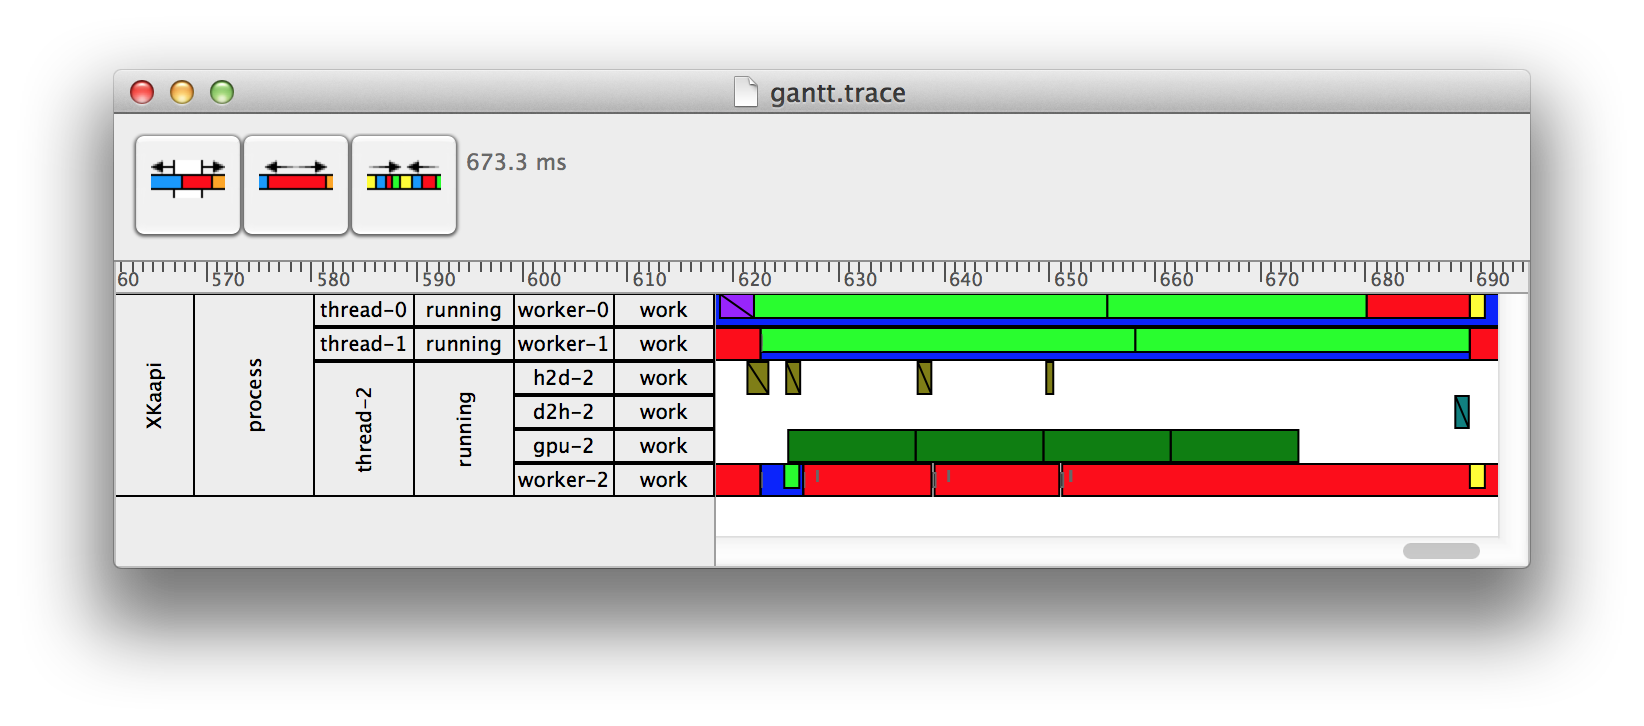
\includegraphics[scale=0.6]{sgemm-paje-trace.png}
\caption{
Gantt diagram of a Paj\'e trace from a \kaapi SGEMM execution with two CPUs and one GPU.
}
\label{fig:trace}
\end{figure}

\definecolor{running}{rgb}{0.0,1.0,0.0}
\definecolor{idle}{rgb}{1.0,0.0,0.0}
\definecolor{active}{rgb}{0.0,0.0,1.0}
\definecolor{unroll}{rgb}{0.6,0.0,1.0}
\definecolor{kernel}{rgb}{0.0,0.5,0.0}
\definecolor{host2device}{rgb}{0.5,0.5,0.0}
\definecolor{device2host}{rgb}{0.0,0.5,0.5}
\definecolor{sync}{rgb}{1.0,1.0,0.0}
%\definecolor{}{rgb}{}

The colors from Figure \ref{fig:trace} represents the states:
\begin{itemize}
\item \textbf{\textcolor{running}{running}} tasks;
\item \textbf{\textcolor{idle}{idle}} state, which means it may request tasks by steal operations, or poll devices such as GPUs;
\item \textbf{\textcolor{active}{active}} state in which the runtime performs other activities as data validation;
\item \textbf{\textcolor{unroll}{unroll}} tasks to the acceleration structure used by \kaapi work stealing algorithm;
\item GPU \textbf{\textcolor{kernel}{kernels}};
\item GPU \textbf{\textcolor{host2device}{host-to-device}} transfers;
\item GPU \textbf{\textcolor{device2host}{device-to-host}} transfers;
\item memory \textbf{\textcolor{sync}{synchronisation}}.
\end{itemize}

We use arrows to illustrate steal request from thief, and reply from its victim. Here we omitted steal events for the sake of space.

% ---------------------------------------------------------------
\section{PAPI performance counters}\label{sec:papi}
% ---------------------------------------------------------------

In \kaapi source files, the example \verb+examples/papi+ shows how to use PAPI
performance counters to measure performance events on a foreach algorithm.
Currently PAPI is supported by the build option \verb+--with-papi+ in which the user
has to give the path of the PAPI library.

The \verb+KAAPI_PERF_PAPIES+ environment variable is used to tell the runtime
which PAPI counters we want to measure. 
An example to measure L1 cache misses, total cycles and FPU operation count is given below:
\begin{verbatim}
> KAAPI_PERF_PAPIES=PAPI_L1_DCM,PAPI_TOT_CYC,PAPI_FP_OPS ./a.out
done: 2797.519360 (ms)
perf_counters: 1048182, 1977006509, 7413173
\end{verbatim}

Some limitations and notes of \kaapi counters with PAPI:
\begin{itemize}
\item limited to up to 3 \verb+KAAPI_PERF_ID_PAPI_x+ counters. See
the man page of \verb+papi_avail(3)+ for a list of supported events.
%\item when using \verb+kaapi_perf_accum_counters+ and equivalent routines, the buffer
% size must be equal the cardinalty of the corresponding \verb+perf_idset+.
\item there is currently no way for the user to define measured sections.
\item it is not possible to dynamically change the event set to measure.
\end{itemize}

\end{document}
